\chapter{Cuts versus the Delphi Principle}
\label{cut}

This chapter discusses the role of the Prolog extra-logical
operator \textit{cut} in pruning the sequential search tree, and
highlights the issues that arise when the tree is searched in
parallel.  Alternative approaches to addressing the issue are
considered.  Gupta and Santa Costa discuss the related issues with AND-OR
parallel Prolog programming in \cite{GSC92}.

%%%%%%%%%%%%%%%%%%%%%%%%%%%%%%%%%%%%%%%%%%%
\section{Cut in standard Prolog programs} %
%%%%%%%%%%%%%%%%%%%%%%%%%%%%%%%%%%%%%%%%%%%
\enlargethispage{2\baselineskip} % manual final formatting

Standard Prolog \cite{DEDC96} provides a built-in extra-logical 
predicate ``cut'' (\texttt{!}/0) aimed at performing some control by
pruning the search tree.  The predicate always succeeds, but has
a drastic effect on the sequential search tree: some branches are
pruned, removing the associated sub-trees, in order to force a predication
to execute more quickly without constructing and visiting those
sub-trees.
The example program containing \textit{cut} from \cite{DEDC96} is
given below:

\begin{minipage}[h]{\textwidth}
\begin{alltt}
p(X,Y) :- q(X), !, r(X,Y).
p(X,Y) :- s(X).\vspace{2mm}
q(a).
q(b).
q(c).\vspace{2mm}
r(b,b1).
r(c,c1).\vspace{2mm}
s(d).\vspace{2mm}
:- p(U,V).
\end{alltt}
\end{minipage}

The AND-OR search tree for this simple example is given in
Figure \ref{cut_and_or_tree}.

\begin{figure}[htb]
\vspace{5mm} \hbox to \hsize{\hfill \psfig{file={cut/ps/cut_and_or_tree.ps}} \hfill}
\caption{The effect of \textit{cut} on the AND-OR search tree.}
\vspace{5mm}
\label{cut_and_or_tree}
\end{figure}

The search tree can be transformed to the OR-only tree given in Figure
\ref{cut_or_only_tree}, more clearly representing the execution
sequence of the Prolog depth-first left-to-right search.  The first
``cut'' encountered prunes the alternative branches to the right of
the current branch, such that only one clause is used to solve
\texttt{p(U,V)} and also only one clause for \texttt{q(U)}.

\begin{figure}[htb]
\vspace{5mm} \hbox to \hsize{\hfill \psfig{file={cut/ps/cut_or_only_tree.ps}} \hfill}
\caption{Effect of \textit{cut} on OR-only search tree.}
\vspace{5mm}
\label{cut_or_only_tree}
\end{figure}

The use of \textit{cut} by a Prolog programmer requires careful
analysis of the sequence in which the search tree is traversed, in
order to ensure the required behaviour is obtained.  The built-in
predicate is often used to enforce determinacy of a relation, usually
within a particular mode of call.  A typical example can be found in
the definition of the relation \texttt{max}:

\begin{verbatim}
max(X,Y,X) :- X > Y, !.
max(X,Y,Y).
\end{verbatim}
The \texttt{max} relation is expected to be used with the first two
arguments instantiated, and the third a variable.  On succeeding, the
third argument will be unified with the larger of the first two
arguments.  The use of cut assumes the top-down, left-to-right
execution of sequential Prolog: \textit{if} the first clause succeeds,
\textit{then} the alternative clause for \texttt{max} will be pruned
from the search.  If the cut were omitted, a goal such as \texttt{:-
max(5,3,X)} would return two answers, \{\texttt{X=5},
\texttt{X=3}\}, and to avoid this problem the relation would be defined
with additional conditional guards:

\begin{verbatim}
max(X,Y,X) :- X > Y.
max(X,Y,Y) :- X =< Y.
\end{verbatim}
Thus the presence of cut has the following implications:
\begin{enumerate}
\item{Subsequent conditions can be omitted from later clauses in the procedure.}
\item{The Prolog system can execute more efficiently by avoiding the construction of
  choice points, unifying the arguments and calling the guard conditions of later clauses.}
\item{The first definition of \texttt{max} which would otherwise return multiple
  solutions is rendered deterministic.}
\end{enumerate}
While the relation \texttt{max} has the required behaviour in the
expected mode, the non-logical definition of the relation can
introduce problems.  If the relation is called with all three
arguments instantiated then unexpected results may be produced.  For
example, with the first definition of \texttt{max} with cut, the goal
\texttt{:- max(5,3,3)} will \textit{succeed}, which might not be what the programmer
expected.  On unification of the
arguments with the head of the first clause, the subgoal \texttt{X >
Y} \textit{fails}, such that the cut is never reached, and execution
continues with the second clause which \textit{succeeds}.

While the use of cut in procedures such as \texttt{max} is a common
programming practice in Prolog, the problems caused can be avoided
with the logical definition given in the second example.  The
deterministic execution of a procedure can be made explicit through
the use of functions, as discussed in detail in Chapter
\ref{functions}, without the use of non-logical relations with cut.

%%%%%%%%%%%%%%%%%%%%%%%%%%%%%%%%%
\section{Experimental Analysis} %
%%%%%%%%%%%%%%%%%%%%%%%%%%%%%%%%%
\label{cut_exp}

The benchmarks used in the earlier analysis of the PrologPF system contain a number
of deterministic relations.  The efficiency of execution can be improved by the
addition of cuts to the programs:
\begin{description}
\item[8 queens and 10 queens: ]{The program used for these benchmarks contains two
  deterministic procedures, \texttt{notthreatened} which succeeds if two pieces are
  not attacking each other and \texttt{safe} which succeeds if a partial board passed
  as an argument has no attacking pieces.  One cut can be inserted into each procedure
  to improve the efficiency of the deterministic execution.}
\item[Pentominoes: ]{This benchmark contains six deterministic procedures, used to
  initialise the board and test the partially filled board for consistency.  The
  introduction of six cuts, one per procedure, makes the determinism explicit to the
  Prolog system for a more efficient execution.}
\end{description}

For the execution of the benchmark programs on a DECStation 3100, Table \ref{cut_counts}
shows the frequency of cuts encountered during the search of each proof tree.

\begin{table}[htbp]
{\small
\begin{tabular}{| l | r | r | r | r |}
\hline
                   & \textbf{Source} & \textbf{Execution} & \textbf{Cuts}        & \textbf{Time}\\
\textbf{Benchmark} & \textbf{Cuts}   & \textbf{Time(ms)}  & \textbf{Encountered} & \textbf{per cut} \\
\hline
\textbf{8-queens}    & 2 &   1898 &  28666 & 66$\mu$s \\
\hline
\textbf{10-queens}   & 2 &  46497 & 814772 & 57$\mu$s \\
\hline
\textbf{Pentominoes} & 6 & 445959 & 197878 & 2.5ms    \\
\hline
\end{tabular}
}
\caption{Count of cuts encountered for the benchmarks on a single cpu.}
\label{cut_counts}
\end{table}

Table \ref{cut_counts} gives the total number of cuts encountered for each benchmark during
the traversal of each search tree.  Using the execution times for the single-cpu case
(Table \ref{single_cpu_table} in Chapter \ref{bfp_depth}), the average period between
each cut can be calculated.  In a parallel processing case this period represents an
upper bound on the average time between the discovery of each cut in the search tree,
and the average will reduce by the speedup factor of a parallel execution.

%%%%%%%%%%%%%%%%%%%%%%%%%%%%%%%%%%%%%%%%%%%%%%%%%%%%%%%%%%%%%%%%%%%%%%%%%%
\section[Strategies for dealing with \textit{cut}]{Strategies for dealing with \textit{cut} in the Delphi Machine} %
%%%%%%%%%%%%%%%%%%%%%%%%%%%%%%%%%%%%%%%%%%%%%%%%%%%%%%%%%%%%%%%%%%%%%%%%%%
\enlargethispage{2\baselineskip} % manual final formatting

The breadth-first partitioning algorithm can be applied to the 
search tree represented in Figure \ref{cut_or_only_tree}.  If the 
partitioning depth limit
is set at a low figure, such as $L=2$, then oracles will be created for the
alternate paths via \texttt{q(U)} and \texttt{s(U)} in the diagram.  If these
oracles are allocated to different path processors, then the discovery of the
cut after the solution of \texttt{q(a)} must be communicated to the path
processor executing the other oracle, such that that search can be aborted.

The path processor searching the subtree to be pruned on the discovery of the
cut may have already communicated solutions to the control processor.

If the system is intended to execute Prolog programs in parallel including
subtrees which may be pruned by cuts discovered by other path processors, then
the simple Delphi system must be extended as follows:
\begin{itemize}
\item{Solutions reported to the control processor must be tagged with the
  associated oracle.}
\item{Any subsequent reporting of a solution to a client program must be delayed until the
  subtrees to the left of the solution in the OR-only tree have been fully
  searched, to ensure the absence of cuts which would otherwise have pruned the
  solution.}
\item{Similarly, the reporting of solutions found within the depth limit during the first phase
  of the scheduling algorithm must be delayed until the left subtrees have been searched.}
\item{The discovery of a cut in a subtree must be communicated to the path processors
  searching subtrees to the right of the discovered cut, such that pruning can be applied.
  However, the communication must be delayed until the subtrees to the \textit{left} of
  the discovered cut have been fully searched to ensure that the subtree containing the
  cut should not itself be pruned.}
\end{itemize}

The pruning of the search tree is limited to the depth of the clause containing the
cut.  The example in Figure \ref{cut_or_only_tree} can be extended with an additional
procedure:
\begin{verbatim}
t(X,Y) :- p(X,Y).
t(a,b).
\end{verbatim}
Figure \ref{cut_or_only_tree2} shows the search tree for the query \texttt{:- t(U,V)}.
The pruning due to the cut in
the OR-only tree beneath \texttt{q(a)} is limited to subtrees
beneath the node labelled \texttt{p(U,V)}.

\begin{figure}[htb]
\vspace{5mm} \hbox to \hsize{\hfill \psfig{file={cut/ps/cut_or_only_tree2.ps}} \hfill}
\caption{Affect of \textit{cut} limited to depth of containing clause in OR-only tree.}
\vspace{5mm}
\label{cut_or_only_tree2}
\end{figure}

In communicating the discovery of the cut to other path processors, an \textit{oracle} can
be used to define the choices affected by the cut.  With reference to 
Figure \ref{cut_or_only_tree2}, on discovering the cut beneath \texttt{q(a)} the path
processor must communicate the oracle referring to the node labelled \texttt{q(U)}. Path
processors receiving the communication must abort any search of subtrees with a prefix
equal or greater to that oracle.  Additional data must be recorded to relate each cut to
the root of the correct subtree in the OR-only tree such that the required oracle
can be created.

Section \ref{cut_exp} shows cuts may be encountered during the execution of a program thousands
or even millions of times each second.  The target architecture for PrologPF assumes a large
supply of processing power with a relatively limited communications capacity.  For this 
reason distributed support for cut was not implemented, and an alternative approach taken.

%%%%%%%%%%%%%%%%%%%%%%%%%%%%
\section{Cuts in PrologPF} %
%%%%%%%%%%%%%%%%%%%%%%%%%%%%

The requirement for ``cut'' in PrologPF is accommodated in two ways:
\begin{enumerate}
\item{Support for higher-order functional programming is provided to mitigate the need for
  cut to provide:
  \begin{itemize}
  \item{Efficient deterministic execution of relations which would otherwise return
    multiple solutions.
    These relations should be replaced with functions in PrologPF.  Functional support in
    PrologPF is discussed in detail in Chapter \ref{functions}.}
  \item{Support for the use of boolean functions, where otherwise the programmer might have
    used the more error-prone negation-as-failure.}
  \end{itemize}}
\item{Cut is permitted in user procedures, but those procedures \textit{must} be deterministic.
  Oracle support is suspended during the execution of procedures containing cut.}
\end{enumerate}

The requirement that the relations containing cut must be deterministic is illustrated by
the search tree for the following program given in Figure \ref{cut_det_tree}.
\begin{verbatim}
t(X,Y) :- p(X,Y), q(X).
t(a,b).

p(X,Y) :- q(X), !, r(X,Y).
p(X,Y) :- s(X).

q(b).
q(c).

r(b,b1).
r(c,c1).

s(d).

:- t(U,V).
\end{verbatim}

\begin{figure}[htb]
\vspace{5mm} \hbox to \hsize{\hfill \psfig{file={cut/ps/cut_det_tree.ps}} \hfill}
\caption{Deterministic execution of a PrologPF relation containing \textit{cut}.}
\vspace{5mm}
\label{cut_det_tree}
\end{figure}

The example program has one solution for the subgoal \texttt{p(U,V)}: \{\texttt{U=b, V=b1}\}.
Oracle processing is suspended during the execution of that subgoal due to the compiler
detection of the cut in the procedure.  When the relation succeeds with its single solution,
oracle processing continues such that the solution to the top-level query has the
oracle \textit{[1,1]}.

Figure \ref{cut_det_tree2} gives the search tree for the same program with the addition of
the clause \texttt{r(b,b2)} at the end of the procedure \texttt{r}, which becomes:
\begin{verbatim}
r(b,b1).
r(c,c1).
r(b,b2).
\end{verbatim}
\begin{figure}[htb]
\vspace{5mm} \hbox to \hsize{\hfill \psfig{file={cut/ps/cut_det_tree2.ps}} \hfill}
\caption{Oracle ambiguity cause by \textit{cut} in a relation with multiple solutions.}
\vspace{5mm}
\label{cut_det_tree2}
\end{figure}

The additional clause for \texttt{r} means that the subgoal \texttt{p(U,V)} has two
solutions \{\texttt{U=b, V=b1}\} and \{\texttt{U=b,V=b2}\} in spite of the presence of
the cut within the procedure for \texttt{p}.  Oracle processing is suspended during the execution
of the subgoal \texttt{p(U,V)}, and restarted on the success of that subgoal.  The
multiple solutions to \texttt{p(U,V)} result in two positions in the search tree having
the same oracle.  The oracle \textit{[1,1]} now refers to the position of both solutions in the
search tree, the ambiguity preventing the use of oracles for parallel partitioning.

It is important to note that the incompatibility of oracles with the use of
cut arises from the subsequent use of
open oracles in the partitioning of the workload among the distributed path processors,
illustrated with the same example in Figure \ref{cut_det_tree3}.

\begin{figure}[htb]
\vspace{5mm} \hbox to \hsize{\hfill \psfig{file={cut/ps/cut_det_tree3.ps}} \hfill}
\caption{Pruned subtree allocation caused by open oracles in relation with \textit{cut}.}
\vspace{5mm}
\label{cut_det_tree3}
\end{figure}

In Figure \ref{cut_det_tree}, at the depth limit $L$ selected, there are three open
oracles: \textit{[1,1,1]},
\textit{[1,1,2]}, and \textit{[1,2,1]}.  The second and third open oracles refer to subtrees that should
be pruned on discovery of the cut in the subtree referenced by the
first oracle.  Suspending oracle processing during the execution of
deterministic procedures containing cut ensures that no open oracle
can be generated within that procedure, potentially referring to a
subtree that would otherwise be pruned by a cut elsewhere in the code.
With the breadth-first partitioning strategy used in PrologPF, each
open oracle is discovered at the fixed depth limit.  The issue of
oracle ambiguity caused by non-deterministic relations containing cut
would be addressed by an extended definition of the depth limit:
\begin{itemize}
\item{Oracle processing continues during the execution of procedures containing cut.}
\item{Forced failure at the selected depth limit in the first phase of breadth-first partitioning
  is deferred until the procedure containing the cut would otherwise succeed.}
\end{itemize}
The second requirement can be viewed as a distortion of the depth limit to include the
entirety of the subtree pertaining to the relation containing the cut.
This approach is illustrated in Figure \ref{cut_det_tree4}.

\begin{figure}[htb]
\vspace{5mm} \hbox to \hsize{\hfill \psfig{file={cut/ps/cut_det_tree4.ps}} \hfill}
\caption{Modified depth limit definition to permit non-deterministic relations with \textit{cut}.}
\vspace{5mm}
\label{cut_det_tree4}
\end{figure}

The support for cut in PrologPF is limited to the simple suspension of oracle processing
while procedures containing cut are executed.  The programmer is responsible for ensuring
those procedures are semi-deterministic, i.e\ have only one solution or \textit{fail}.
No parallel speedup is available
to procedures containing cut, and the functional support is provided to render the
deterministic execution of those algorithms explicit.

%%%%%%%%%%%%%%%%%%%%%%%
\section{Conclusions} %
%%%%%%%%%%%%%%%%%%%%%%%

The simple distributed implementation of the \textit{cut} extra-logical relation would require
the communication of the discovery of the cut to all path processors searching affected
subtrees.  Oracles can be used to identify the subtrees affected by the cut, but the
communication requirements to support the distribution of the pruning information could
be substantial.  This distributed implementation is unsuited to the target architecture for
PrologPF, in which many general purpose processors are loosely coupled with a local- or
wide-area network.

Cuts can be accommodated within the distributed processing framework of PrologPF by modifying
the oracle management algorithms and depth limit processing within procedures containing
cut.  The PrologPF compiler recognises cut within user procedures, and disables oracle
processing during the execution of those procedures.  The techniques discussed do not permit
parallel speedup of procedures containing cut.

PrologPF aims to minimise the requirement for cut by providing support for higher-order
functional programming, discussed in detail in the next chapter.

%%%%%%%%%%%%%%%%%%%
\section{Summary} %
%%%%%%%%%%%%%%%%%%%

Standard Prolog \cite{DEDC96} provides a extra-logical predicate ``cut''
(\texttt{!}/0) which always succeeds, but has the side effect of
removing following alternative subtrees from the problem search tree.
The semantics of cut are dependent upon the depth-first, left-to-right
execution semantics of sequential Prolog.

Procedures containing the special predicate ``cut'' are often designed to be used within
a particular \textit{mode}, in which some arguments are expected to be instantiated at
the time of the call while other are expected to contain logical variables.  The use
of procedure with a different pattern of instantiated and uninstantiated arguments can
lead to unintended results.  The use of cut within Prolog programs is a common
source of error.

The benchmark programs used in the analysis of the distributed performance of PrologPF
contain some deterministic procedures with cuts.  Run-time analysis on a single cpu
showed that the cuts were encountered in those sample programs between 400 and 18000 times
each second.  The simple implementation on multiple cpu's would be expected to increase
that rate.

Oracles could be used to support a distributed implementation of the cut predicate, in
which the subtrees to be pruned are identified with the associated oracle to be propagated
to the affected path processors.

The target architecture for the distributed execution of PrologPF programs has a relatively
high cost of communication, in contrast to an abundance of processing power within each
distributed path processor.  For this reason, simple support for cut is provided in which
oracle processing is suspended during execution of procedures containing cut.  This prevents
the discovery of open oracles within any procedure containing cut. No oracles
referring to a subtree within the search tree of a procedure containing cut can be generated
by PrologPF, and so cannot be allocated for processing in a separate path processor.

In PrologPF, procedures containing cut must be deterministic to avoid ambiguity of the
oracles skipping over the subtrees of those procedures.  A modification to the definition
of the depth limit used in the breadth-first partitioning strategy of PrologPF would remove
that limitation.

The use of the predicate ``cut'' in PrologPF programs can often be
avoided through the use of higher-order functional programming, a
technique not available to programmers of standard Prolog.
This approach forms the subject of the following chapter.



